\documentclass[conference]{IEEEtran}
\IEEEoverridecommandlockouts
% The preceding line is only needed to identify funding in the first footnote. If that is unneeded, please comment it out.
\usepackage{cite}
\usepackage{amssymb,amsfonts, mathtools}
\usepackage{amsmath}
\interdisplaylinepenalty=2500
\DeclareMathOperator{\sgn}{sgn}
\DeclarePairedDelimiter{\ceil}{\lceil}{\rceil}
\DeclarePairedDelimiter{\floor}{\lfloor}{\rfloor}
\usepackage{algorithmic}
\usepackage[serbian]{babel}
\usepackage{graphicx}
\usepackage{textcomp}
\usepackage{hyperref}
\usepackage{xcolor}
\def\BibTeX{{\rm B\kern-.05em{\sc i\kern-.025em b}\kern-.08em
		T\kern-.1667em\lower.7ex\hbox{E}\kern-.125emX}}

% --------------------------------------------------------------------------------------
\begin{document}

\title{Sistem za direktnu digitalnu sintezu}

\author{\IEEEauthorblockN{Kristijan Mitrović}
\IEEEauthorblockA{\textit{Odsek za elektroniku} \\
	\textit{Elektrotehnički fakultet}\\
	Beograd, Srbija \\
	mk150214d@student.etf.bg.ac.rs}
\and
\IEEEauthorblockN{ Dragan Božinović}
\IEEEauthorblockA{\textit{Odsek za elektroniku} \\
	\textit{Elektrotehnički fakultet}\\
	Beograd, Srbija \\
	bd150211d@student.etf.bg.ac.rs}
}

\maketitle

% -------------------------- Abstract ------------------------------------------------
\begin{abstract}
Ovaj rad predstavlja opis rešenja projekta iz predmeta \textit{Hardversko-softverska obrada signala}. Dat je pregled realizovanih funkcionalnosti uz potrebne teorijske temelje nužne za razumevanje odabrane implementacije.
\end{abstract}
% ------------------------- Razvojno okruženje ---------------------------------------------------
\section{Razvojno okruženje}
Programski kod koji obavlja zahtevanu funkcionalnost sistema napisan je u programskom jeziku \textit{C++}, dok je razvojno okruženje korišćeno za izradu ovog projekta \textit{Visual Studio Code}.

Za potrebe fiksne aritmetike korišćene su biblioteke \texttt{ac\_fixed.h} i \texttt{ac\_int.h}, pri čemu prva omogućava rad sa brojevima sa fiksnim zarezom dok druga biblioteka služi za korišćenje celobrojnih promenljivih ograničenih na određen broj bita.

Funkcionalnost je ostvarena u okviru fajla ''\textit{main.cpp}``. Vrednosti koje se po uslovu zadatka vode na DAC konvertor i određeni međurezultati bivaju smešteni u fajl ''\textit{DDSlog.csv}``, dok fajl ''\textit{logProcess.m}`` predstavlja skriptu koja se pokreće iz \textit{MATLAB}-a i služi za prikaz rezultata smeštenih u okviru \textit{log} fajla.

\section{Funkcionalni blokovi sistema}
% ------------------------- W ---------------------------------------------------
\subsection{Fazni akumulator}
Fazni akumulator realizovan je u vidu promenljive \texttt{phaceAcc}. Ova promenljiva, budući da je ograničena širinom od $W=40$ bita, predstavlja broj u opsegu $[0, 2^{40}-1]$. Frekvencija generisanog signala određena je inkrementom faznog akumulatora, označenog sa \texttt{dteta}, pri čemu minimalna vrednost inkrementa predstavlja frekvencijsku rezoluciju. Ipak, budući da su obe promenljive bezdimenzioni brojevi, omogućena je intuitivna manipulacija ovim vrednostima. Imajući u vidu da je najmanji inkrement faznog akumulatora jednak $\Delta \theta_{min}$ = $2^0$ = $1$, \texttt{dtheta} se računa po formuli
\\
\begin{equation}
\Delta \theta = M_{inc}\,\Delta \theta_{min} = \frac{f_0}{\Delta f} = \frac{f_{0}}{f_{clk}}\,2^W ,
\end{equation}

\noindent pri čemu je sa $f_{o}$ označena učestanost željenog signala a sa $f_{clk}$ učestanost takta. Ovakvim pristupom, korisniku je omogućeno da unese željenu frekvenciju u vidu promenljive \texttt{f0} koja nadalje biva skalirana u odgovarajući inkrement faznog akumulatora, čime u potpunosti biva lišen unošenja neintuitivnih brojeva. Ujedno je i  za najmanju ostvarivu frekvenciju, $\Delta f$, inkrement faznog akumulatora jednak bitu najmanje težine, čime je postignuta uniformna kvantizacija faznog akumulatora, odnosno, pri ovoj učestanosti kvantizacioni šum ne postoji. Maksimalna ostvariva učestanost ovakvog sistema, $f_s/2$, biva preslikana u inkrementalni pomeraj od $2^{W-1}$, odnosno, u pomeraj koji je jednak $\pi$.

Početna faza, označena sa \texttt{phi}, predstavlja takođe ceo broj dužine $W=40$ bita. Korisnik unosi željenu početnu fazu preko promenljive \texttt{phi0}, pri čemu njena vrednost pripada intervalu $[0, 2\pi]$. Tako unesena vrednost se dalje skalira: kako maksimalni pomeraj od $2^W$ odgovaraja inkrementu faze za $2\pi$, to znači da za $\phi_0 = 2\pi$ inkrement akumulatora mora biti jednak $2^W$. Stoga, početna faza koja se pridodaje faznom akumulatoru računa se po formuli

\begin{equation}
	\phi = \frac{\phi_0}{2\pi} 2^W
\end{equation}

Na slici \ref{slika:kos1} prikazan je kosinusoidalni signal čija je učestanost $f_0 = 1$\, MHz. 

\begin{figure}[h]
	\centering
	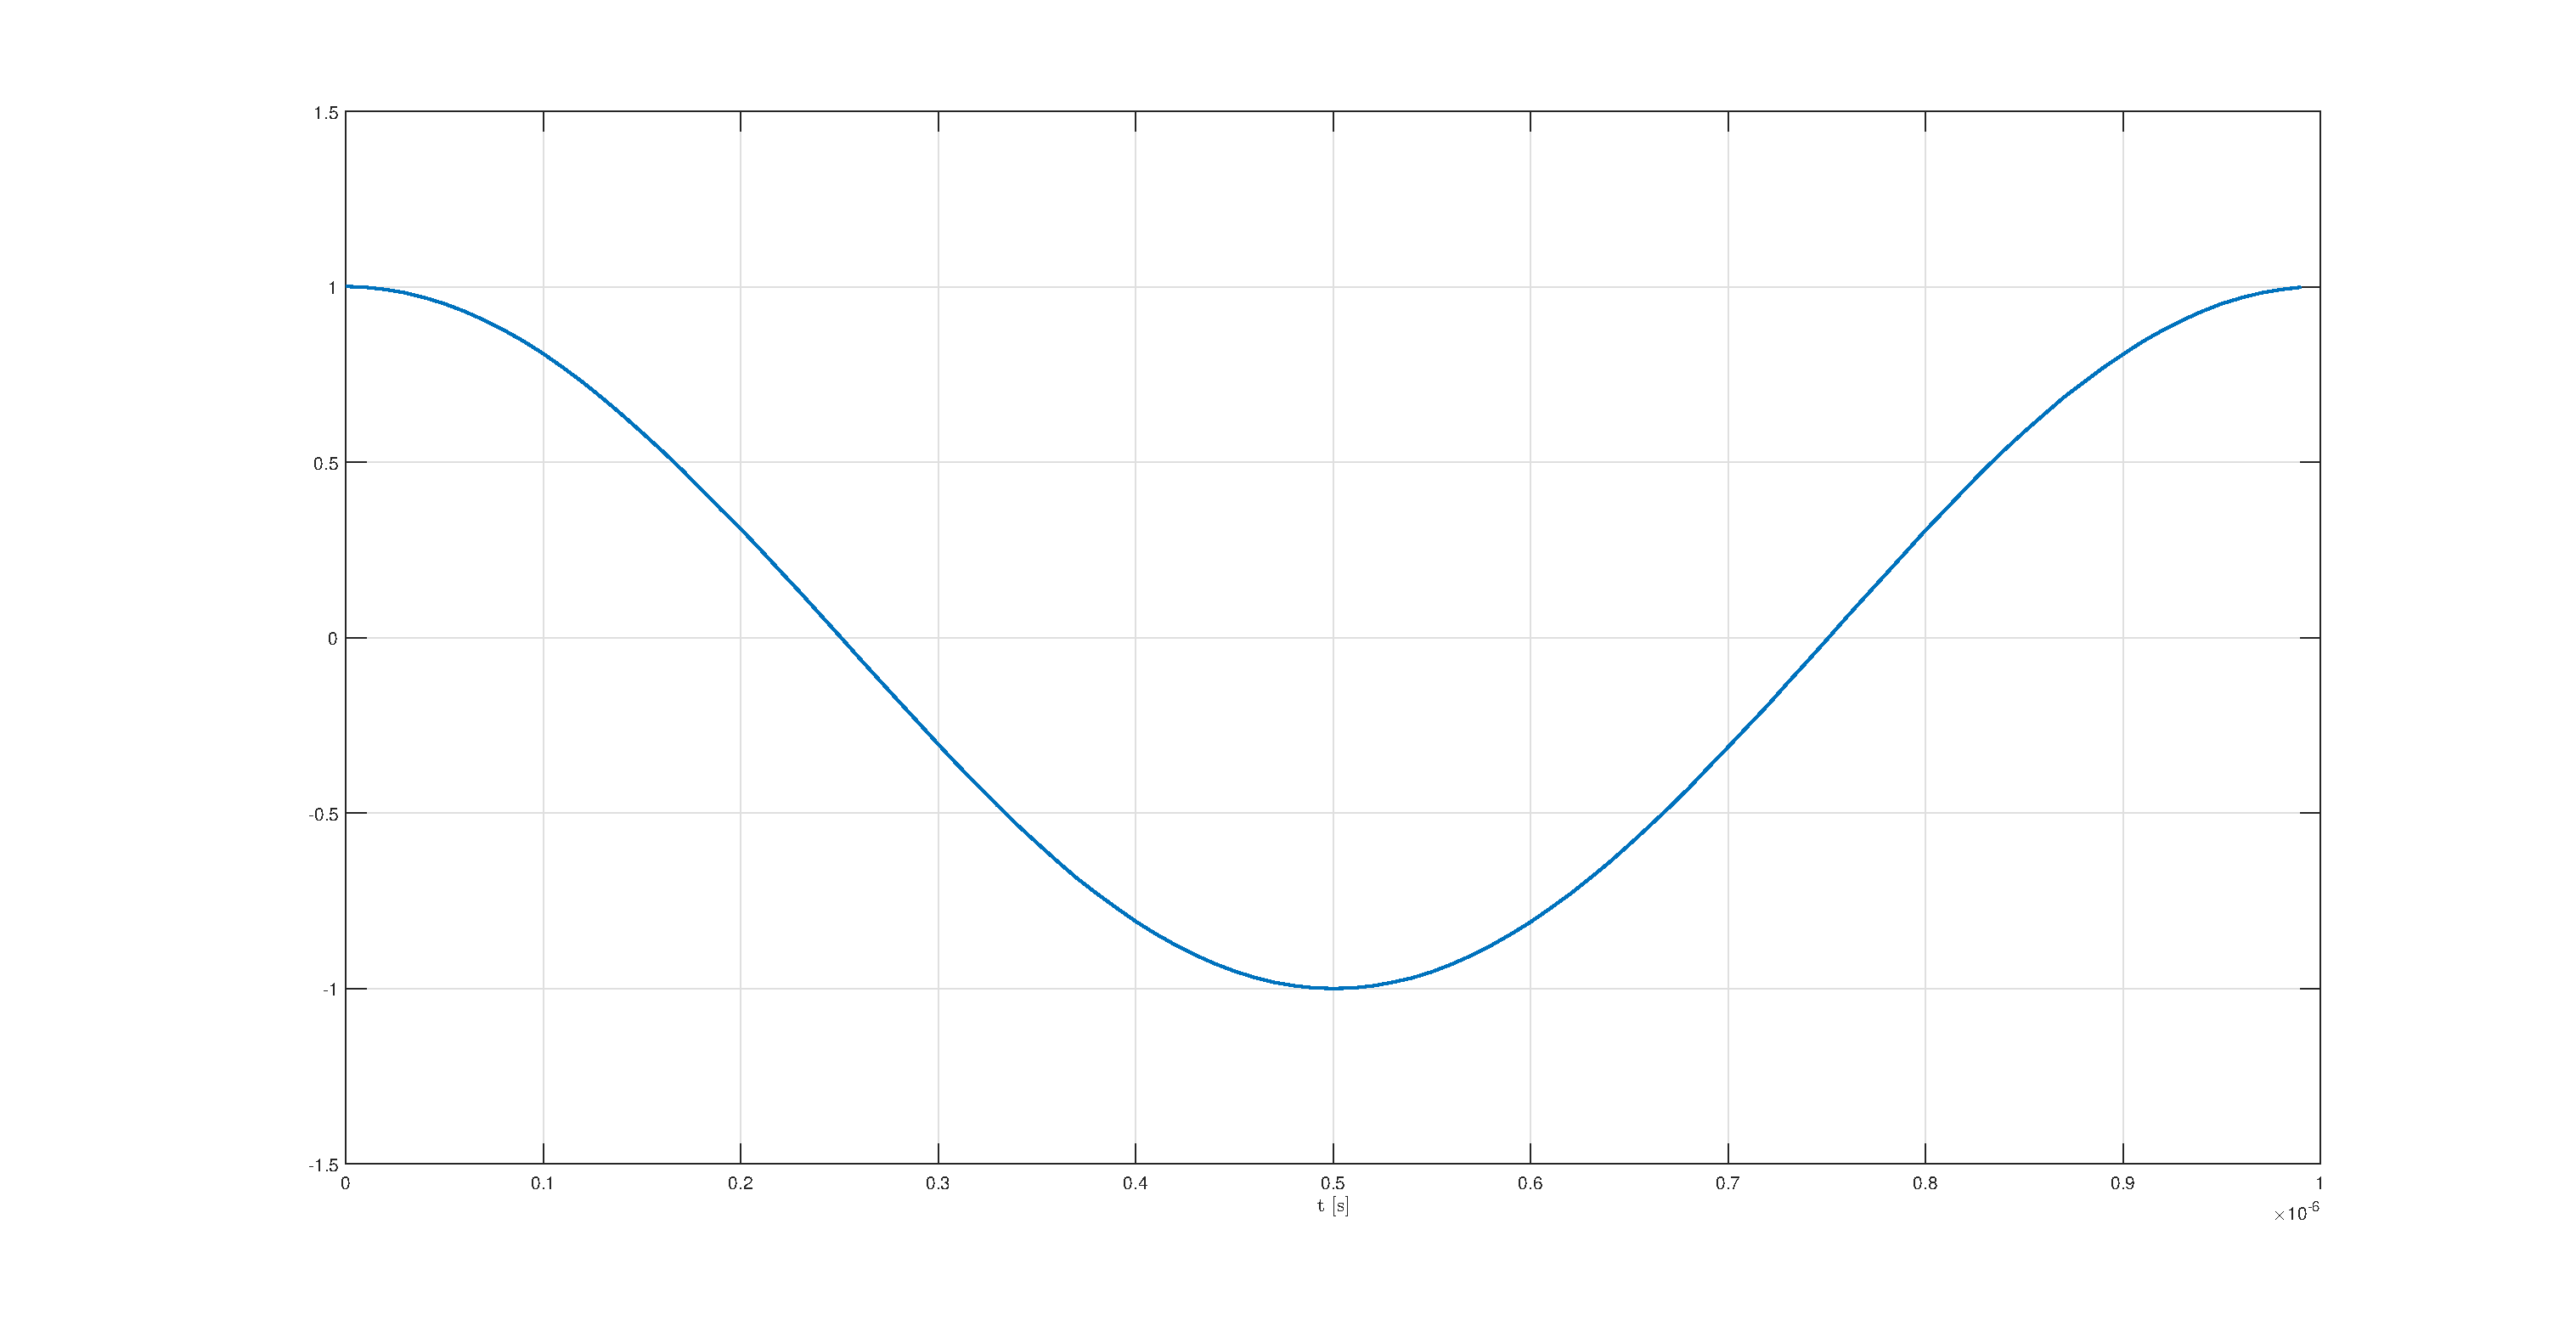
\includegraphics[scale=0.15]{./slike/kos1.eps}
	\caption{\textsl{Kosinus učestanosti 1\,MHz}}
	\label{slika:kos1}
\end{figure}

Promenom korisnički definisanih parametara na $f_0 = 2$\, MHz i $\phi_0 = \pi/4$ dobija se kosinusoida prikazana na slici \ref{slika:kos2}. Kao što se da videti, učestanost kosinusoide je duplo veća, pri čemu je izvršen fazni pomeraj koji je unet od strane korisnika.

\begin{figure}[h]
	\centering
	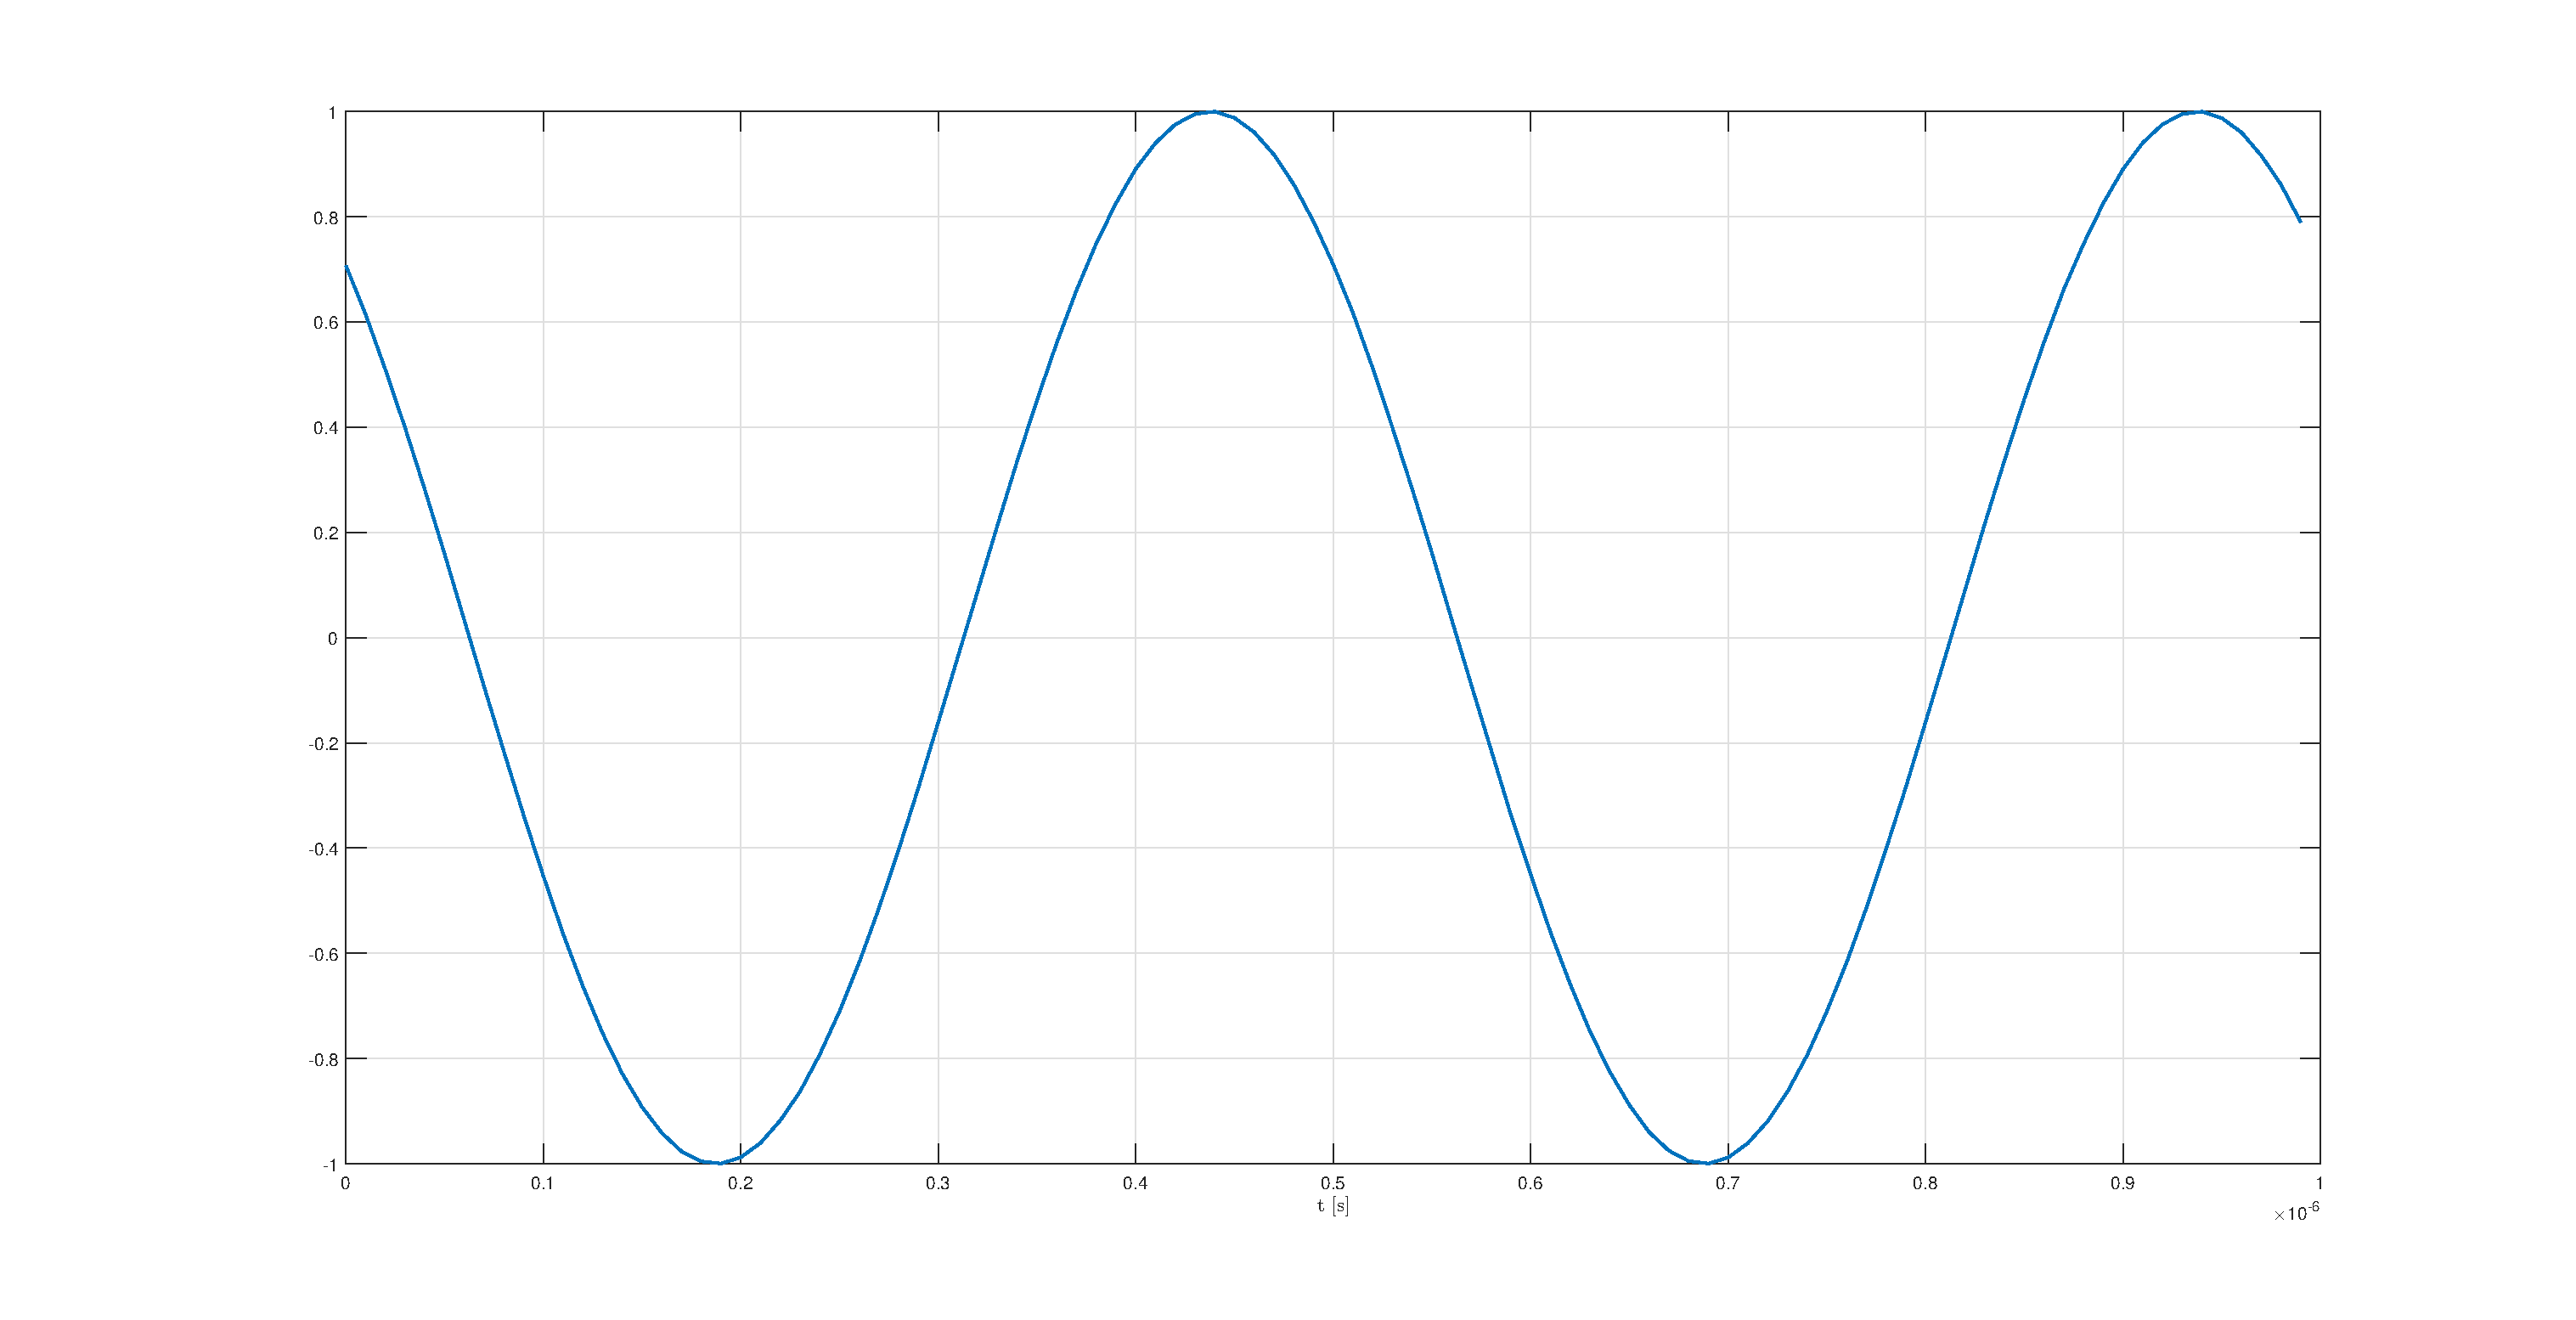
\includegraphics[scale=0.15]{./slike/kos2.eps}
	\caption{\textsl{Kosinus učestanosti 2\,MHz i početne faze $\pi$/4}}
	\label{slika:kos2}
\end{figure}
\pagebreak

% ------------------ cos x -------------------------------------------
\subsection{Generator odbiraka $cos\,x$}
Izlaz iz faznog akumulatora, promenljiva \texttt{phaseAccOut}, dovodi se na ulaz u \textit{CORDIC} algoritam, gde je nadalje potrebno izračunati vrednost amplitude na osnovu dovedene vrednosti. S obzirom na to da se vrednosti iz \textit{CORDIC} algoritma prosleđuju DA konvertoru, odnosno, da je broj različitih vrednosti koje DAC može prihvatiti jednak $2^{14}$, proizilazi da je broj bita koji treba proslediti ovoj tabeli jednak $M=N=14$.

Kako je maksimalna vrednost ugla koja se može proslediti \textit{CORDIC} algoritmu jednaka $99.88$\textdegree, potrebno je na neki način ograničiti vrednost ugla koja se prosleđuje za izračunavanje amplitude. To je učinjeno tako što se najviših dva bita dovodi na ulaz multipleksera u vidu promeljive \texttt{muxSel}, dok se ostalih $12$ bita koristi za mapiranje vrednosti u opsegu od $[0, \frac{\pi}{2}]$ u vidu \texttt{phaseAccOut}.

\textit{CORDIC} algoritam izvršava se u rotacionom modu u \textit{M} iteracija, a po sledećoj formuli:

\begin{eqnarray}\label{kordik}
x_{i+1} &=& x_i - \sigma_i y_i \gg i 		\\
y_{i+1} &=& y_i + \sigma_i x_i \gg i 		\\
z_{i+1} &=& z_i - \sigma_i\arctan{2^{-i}}		\\
\sigma_i &=& \sgn(z_i)
\end{eqnarray}

Radi optimizacije, pre samog početka rada napravljena je svojevrsna tabela vrednosti za $\arctan{2^{-i}}$. Budući da se taj niz vrednosti pojavljuje u svakoj iteraciji faznog akumulatora, ovim je postignuta manja redudansa kao i brže izvršavanje samog programa.

Ipak, kako kontrolna promenljiva na ulazu u \textit{CORDIC} tabelu, \texttt{phaseAccOut}, nema nikakvu realnu dimenziju, potrebno je izvršiti skaliranje. Budući da je maksimalna vrednost \texttt{phaseAccOut} jednaka $2^{M-2}-1$ i da ona odgovara fazi od $\pi/2$, promenljiva \texttt{z} se računa po formuli:

\begin{equation}
z = \frac{phaseAccOut}{2^{M-2}-1} \frac{\pi}{2}
\end{equation}

Izlazne vrednosti, $x$ i $y$, smeštaju se zatim u promenljive \texttt{sampleSin} i \texttt{sampleCos}, na osnovu vrednosti promenljive \texttt{muxSel}.

ZAŠTITNI BITI?

% ------------------------- Diter -----------------------------------------
\subsection{Diter}
Spurovi se javljaju kao neželjene periodične smetnje u spektru izlaznog signala i posledica su neuniformne kvantizacije faze. Pri koherentnom odabiranju uslovljenom jednačinom

\begin{equation}\label{eq:koher}
\frac{f_{0}}{f_{clk}} = \frac{P}{M}
\end{equation}

\noindent gde je $f_{0}$ željena učestanost signala, $f_{clk}$ učestanost odabiranja, $P$ paran broj, a $M=2^m$ broj odbiraka, spurovi su jasno vidljivi u spektru signala, kao na slici \ref{slika:spur}.

\begin{figure}[h]
	\centering
	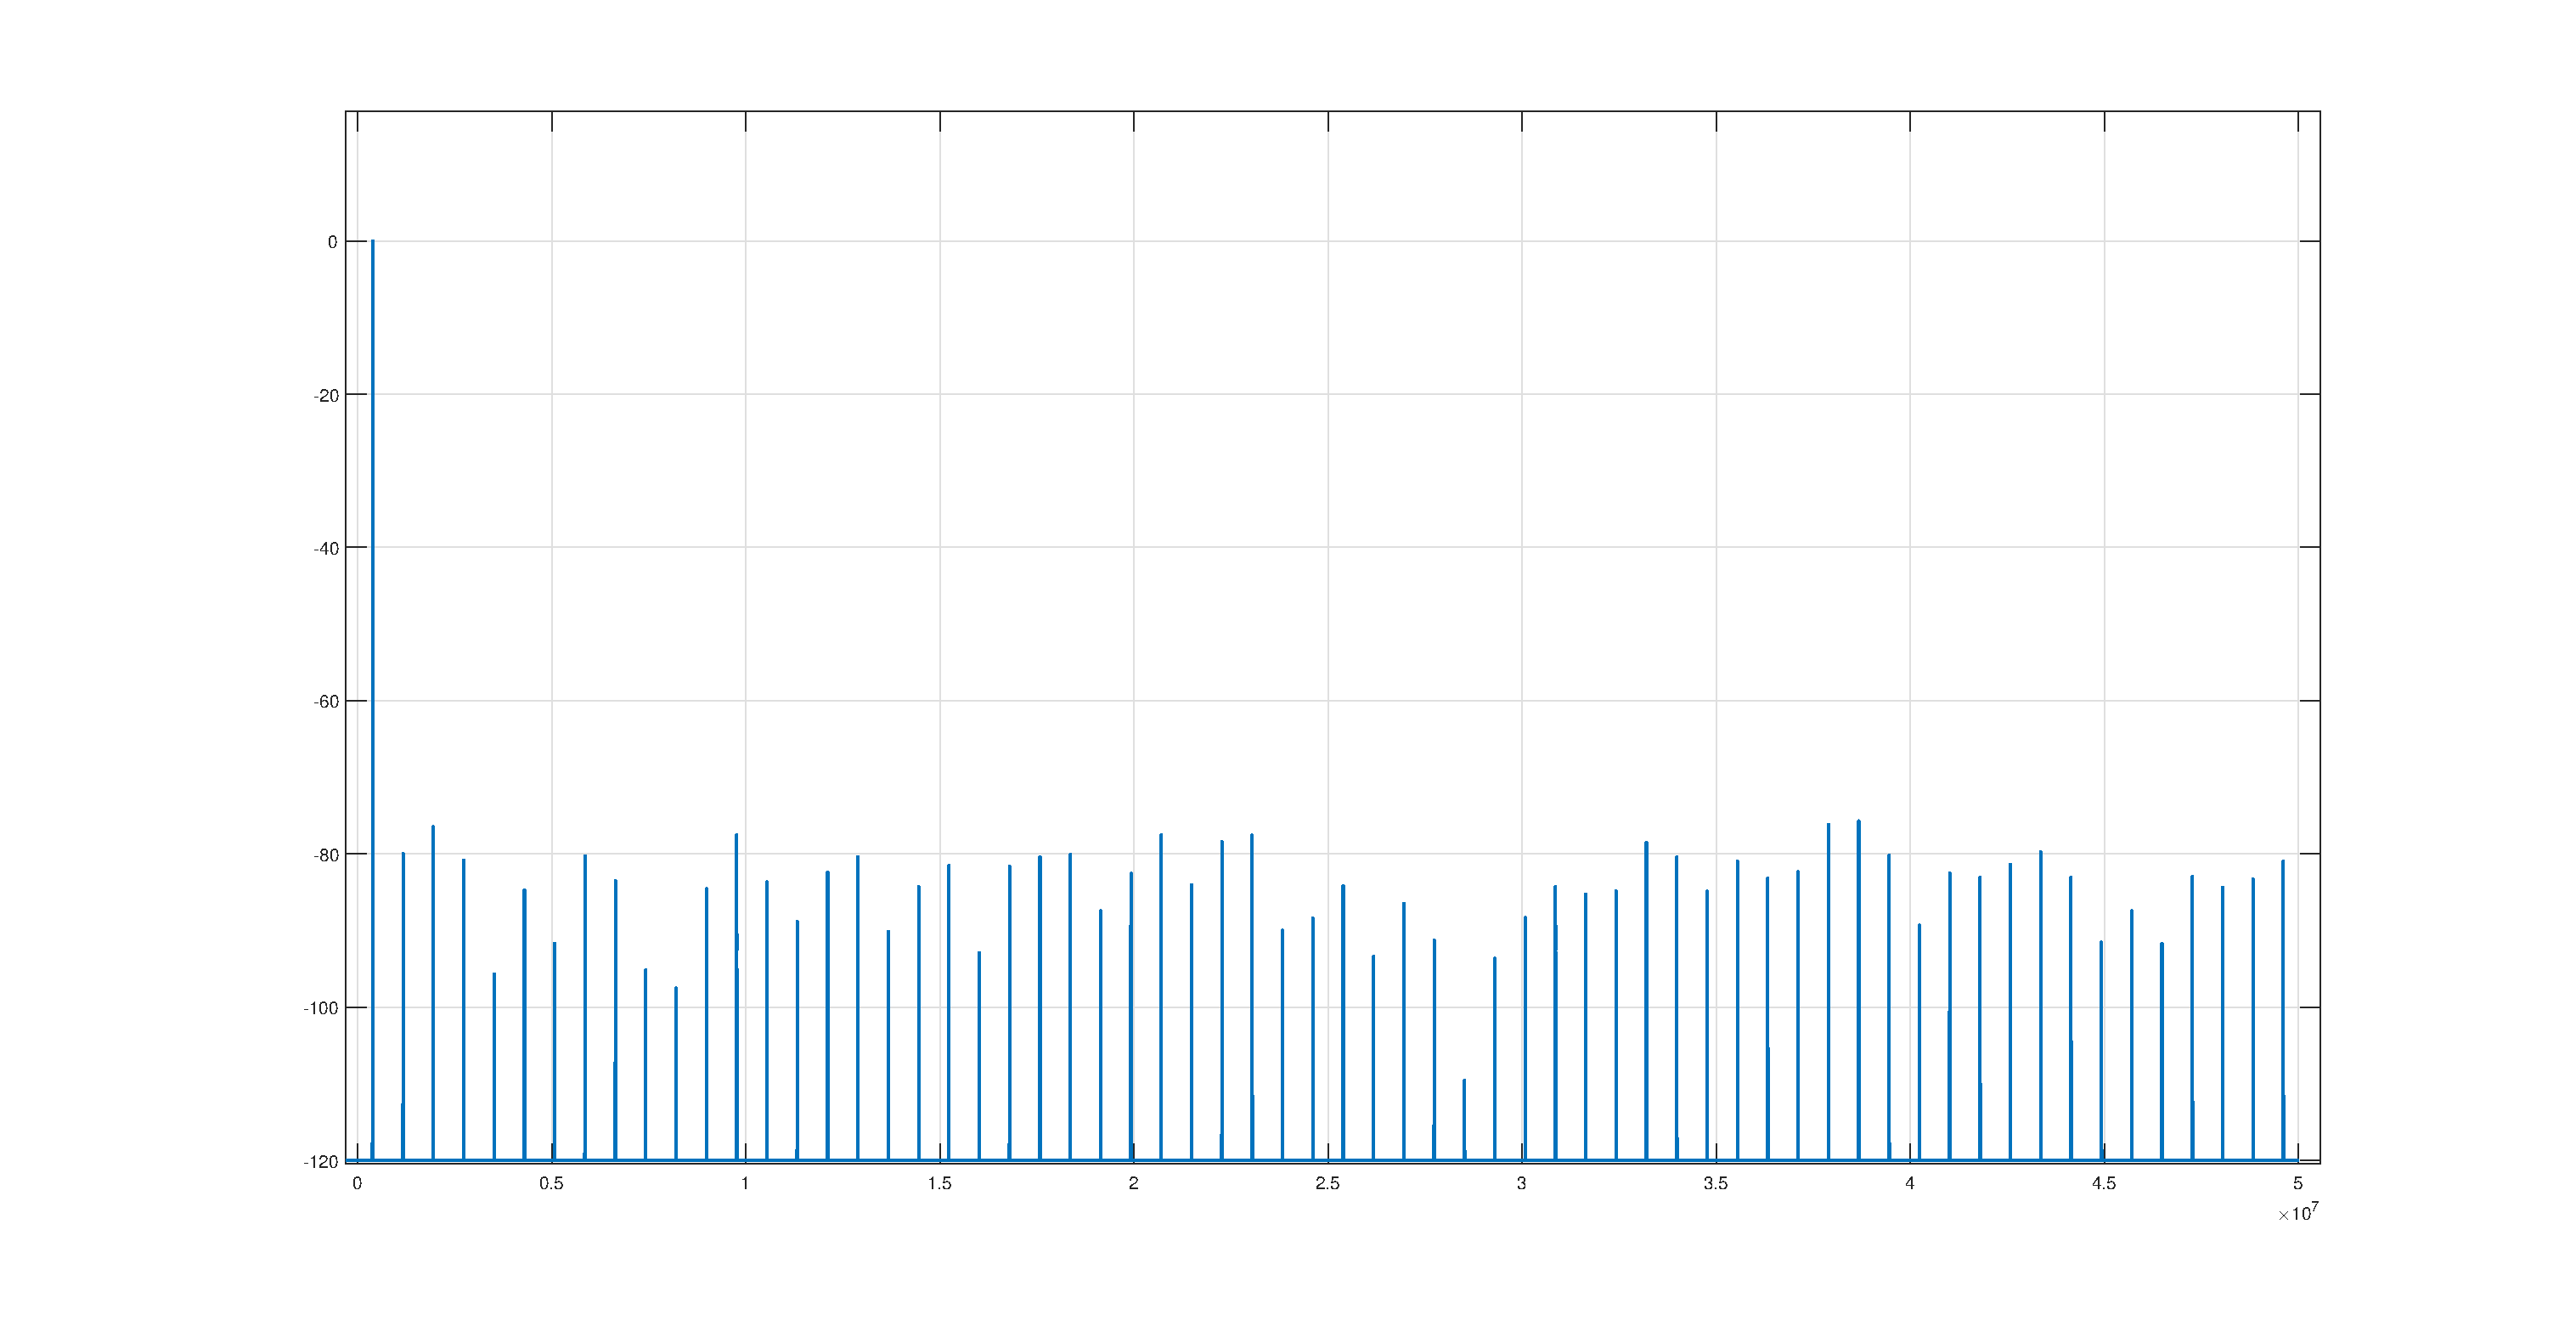
\includegraphics[scale=0.15]{./slike/spur.eps}
	\caption{\textsl{Spektar izlaznog signala u kom su vidljivi spurovi}}
	\label{slika:spur}
\end{figure}

Taktovanje celog sistema u \textit{C++}-u implementirano je \texttt{for} petljom koja se, na osnovu jednačine (\ref{eq:koher}), izvršava $2^n$ puta. U implementaciji je uzeto da je $n=16$, koje obezbeđuje izuzetno brzo izvršavanje programa u \textit{C++}-u, dok, s druge strane, \textit{MATLAB}-u pruža dovoljan broj odbiraka za detaljno iscrtavanje signala i njegovog spektra. Naravno, ovo uzrokuje da je frekvencijski bin u \textit{MATLAB}-u širine $\Delta f=f_{clk}/2^{16}$, a ne $\Delta f=f_{clk}/2^{40}$, ali je dovoljno dobar kompromis između oprečnih zahteva za preciznošću i kratkim vremenom izvršavanja.

Tehnika koja je iskorišćena za razbijanje spurova je tzv.~\textit{ditering}. Ova tehnika sastoji se od dodavanja nekorelisanog ili pseudoslučajnog signala na ''spurovit`` signal, čime se razbijaju periodične komponente. Pseudoslučajan signal u \textit{C++}-u implementiran je instanciranjem objekata \texttt{default\_random\_engine} i \texttt{normal\_distribution} iz \texttt{<random>} biblioteke, koji omogućavaju generisanje slučajnih brojeva sa normalnom raspodelom $\mathcal{N} {\raise.17ex\hbox{$\scriptstyle\mathtt{\sim}$}} (\mu, \sigma^2)$ sa proizvoljnim $\mu$ i $\sigma$. Generisani pseudonasumični brojevi sa $\mu=0$ i $\sigma=1$ pomnoženi su sa $2^{26}$ kako bi se šiftovali do bita koji se prosleđuju \textit{CORDIC} algoritmu, kao i sa \texttt{ditherAmp} čime se podešava nivo ditera koji se dodaje na fazni akumulator u svakoj iteraciji pomenute \texttt{for} petlje.\pagebreak

Na slici \ref{slika:nospur} prikazan je spektar izlaznog signala popravljen nesupstraktivnim diterom, na kom se više ne uočavaju spurovi.

\begin{figure}[h]
	\centering
	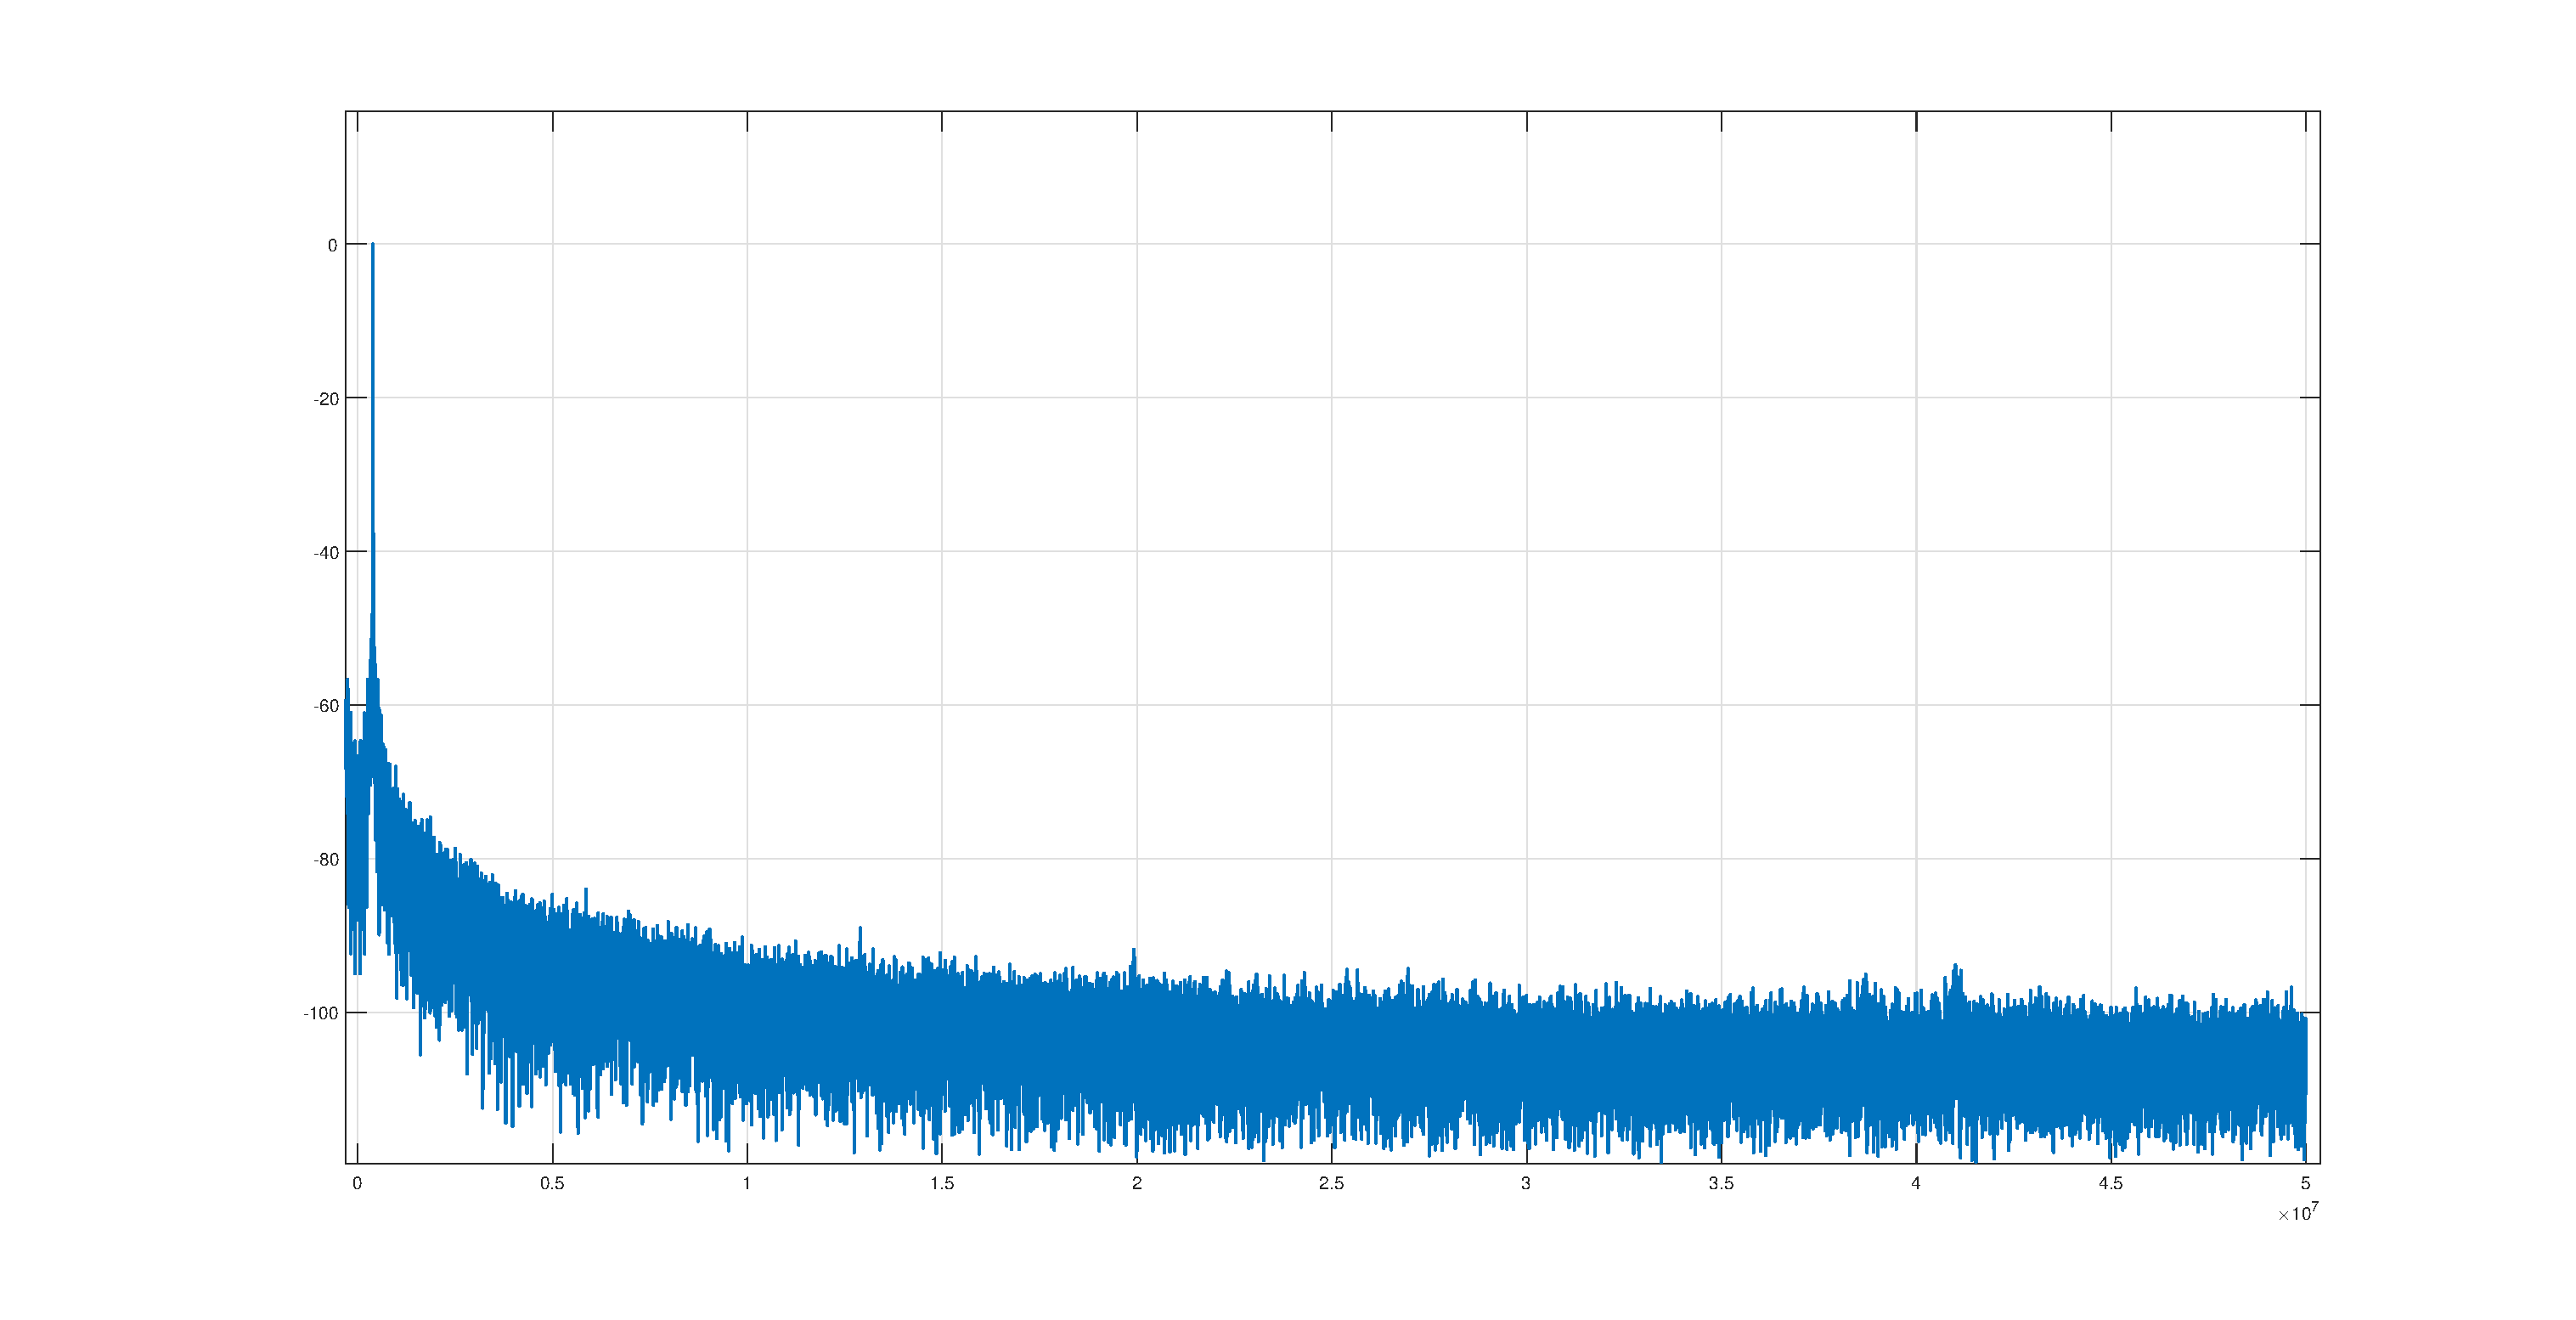
\includegraphics[scale=0.15]{./slike/nospur.eps}
	\caption{\textsl{Spektar izlaznog signala bez spurova}}
	\label{slika:nospur}
\end{figure}

% ------------------------- FIR -----------------------------------------
\subsection{FIR filtar}
FIR filtar za korekciju $\sin x/x$ frekvencijske karakteristike kola zadrške nultog reda implementiran je direktnom realizacijom sa slike \ref{slika:FIRreal}.

\begin{figure}[h]
	\centering
	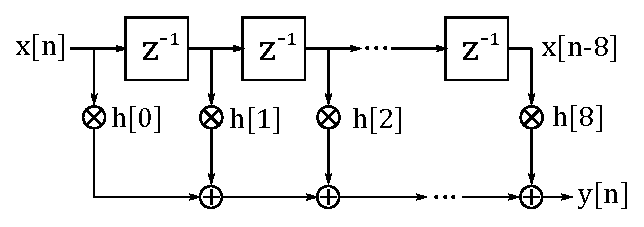
\includegraphics[scale=0.7]{./slike/FIRreal.eps}
	\caption{\textsl{Direktna realizacija FIR filtra}}
	\label{slika:FIRreal}
\end{figure}

Prethodni sistem može se matematički zapisati kao

\begin{equation}\label{eq:konv}
y[n] = \sum_{i=0}^{8}{h[i]\,x[n-i]}
\end{equation}

\noindent što predstavlja konvoluciju koeficijenata filtra $h[0]\ldots h[8]$ sa trenutnim $x[n]$ i prethodnim $x[n-1]\ldots x[n-8]$ izlazima \textit{CORDIC}-a.

Na identičan način je u nizove \texttt{cordicSin} i \texttt{cordicCos} smeštano poslednjih devet izlaza generatora odbiraka, i ti nizovi su po jednačini (\ref{eq:konv}) konvoluirani sa koeficijentima filtra prethodno izračunatim u \textit{Python}-u tako da filter zadovoljava zahtevane uslove, i smeštenim u \texttt{filter} niz. Rezultati konvolucije, tj.~filtriranja \texttt{DACinputCos} i \texttt{DACinputSin} potom su upisani u izlazni fajl za logovanje.

\newpage

% ------------------ Reference ---------------------------
\begin{thebibliography}{00}
	\bibitem{b1} Dr.~Dušan Grujić, Predavanja iz predmeta \textsl{Hardversko-softverska obrada signala}, Elektrotehnički fakultet, Beograd\\
	\bibitem{b2} Bruce Land, \textsl{Direct Digital Synthesis}, Cornell University, New York, \\\url{https://www.youtube.com/watch?v=YDC5zaEZGhM}\\
	\bibitem{b3} Analog Devices, \textsl{Fundamentals of Direct Digital Synthesis}, \\\url{https://www.analog.com/media/en/training-seminars/tutorials/MT-085.pdf}\\
	\bibitem{b4} HLS LIBS, \textsl{AC DATATYPES}, \\\url{https://hlslibs.org/#collapseACDatatypes}\\
	\bibitem{b5} C++, \textsl{std::normal\_distribution}, \\\url{http://www.cplusplus.com/reference/random/normal_distribution/}\\
\end{thebibliography}


\end{document}